\documentclass[12 pt]{article}

\usepackage[utf8]{inputenc}
\usepackage[T1]{fontenc}

\usepackage{amssymb,amsmath}
\usepackage{textcomp}
\usepackage{mathtools}
\usepackage{enumitem}
\usepackage{bm}	% In order to have bold italic in math mode
\usepackage{todonotes}	% In order to have clean todo's
\usepackage[labelfont=bf]{caption}
\usepackage{subcaption}
\usepackage{graphicx}
\usepackage{epstopdf}
\usepackage[colorlinks=true,linkcolor=red]{hyperref}
\usepackage{cleveref}


\begin{document}

\begin{titlepage}
    \vspace{-1cm}
    
    \begin{minipage}{0.6\textwidth}
        \begin{flushleft}
            \centering
            \textsc{University of Liège} \\
            \textsc{Faculty of Applied Sciences} \\
            \textsc{Academic Year 2017 - 2018}
        \end{flushleft}
    \end{minipage}

    \vspace{-2.6cm}
    \hspace{0.5\textwidth}
    
    \begin{minipage}[t]{1.1\textwidth}
        \begin{flushright}
            \includegraphics[scale=0.15]{uLIEGE_Faculte_SciencesAppliquees_Logo_CMJN_pos}
        \end{flushright}
    \end{minipage}

    \vspace{1cm}


    \begin{minipage}{\textwidth}
        \hspace{-0.7cm}\noindent\makebox[\linewidth]{\rule{\textwidth}{2pt}} 
    \end{minipage}

    \vspace{1cm}

    \begin{minipage}{\textwidth}
        \begin{center}
           \hspace{-0.8cm}\Huge{\textsc{\textbf{MATH0471-Multiphysics Integrated Computational Project}}}\\
            \vspace{0.3cm}
            \hspace{-0.8cm}\textsc{C. GEUZAINE \\ R. Boman} \\
        \end{center}
    \end{minipage}

    \vspace{1cm}

    \begin{minipage}{\textwidth}
        \hspace{-0.7cm}\noindent\makebox[\linewidth]{\rule{\textwidth}{0.2pt}}
    \end{minipage}

    \vspace{1cm}

    \begin{minipage}{\textwidth}
        \begin{center}
            \hspace{-1cm}\Huge{\textbf{Intermediate report 1}} \\ 
            \vspace{0.5cm}
        \end{center}
    \end{minipage}

    \vspace{1cm}

    \begin{minipage}{\textwidth}
        \hspace{-0.7cm}\noindent\makebox[\linewidth]{\rule{\textwidth}{0.2pt}}
    \end{minipage}

    \vspace{1cm}

    \begin{minipage}{\textwidth}
        \begin{center}
            \hspace{-1cm}\large{\textsc{DELCOURT Arnaud}} \\
            \hspace{-1cm}\large{\textsc{DESSERS Christophe}} \\
            \hspace{-1cm}\large{\textsc{HEUCHAMPS Alexandre}} \\
            \hspace{-1cm}\large{\textsc{TOMASETTI Romin}} \\
            \vspace{1cm}
            \hspace{-1cm}\Large{\textsc{\today}} \\
        \end{center}
    \end{minipage}
    
    \vspace{1cm}
    
    \begin{minipage}{\textwidth}
        \hspace{-0.7cm}\noindent\makebox[\linewidth]{\rule{\textwidth}{2pt}}
    \end{minipage}
\end{titlepage}

\tableofcontents
\newpage
\listoffigures
\newpage
\listoftables
\newpage

% \section{Questions to ask on February, 20}

% \begin{itemize}
% 	%
% 	\item Do we have to take into account the frequency-dependency of the electromagnetic properties of the materials? (see \url{https://em.geosci.xyz/content/physical_properties/magnetic_permeability/magnetic_permeability_frequency_dependent.html})
% 	%
% 	\item Regarding the already-written code:
% 		\begin{itemize}
% 			\item Comments on the created classes?
% 			\item Is speed affected? Or we don't care?
% 			\item Especially, ask if Array\_3D\_Template<Node> nodes is a good way to start !
% 		\end{itemize}
% 	%
% 	\item Regarding testing, what are the simplest tests? Could we compare our results with other simulations? Do we have to compare with something that can be hand-solved?
% 	%
% 	\item Check our reasoning on the nodes. They all have:
% 		\begin{itemize}
% 			\item 3 coordinates (3 doubles) - How are we going to mesh ??? (we think we are obliged to keep rectangular parallelepiped because of the numerical scheme)
% 			%
% 			\item 6 fields (3 for $\vec{E}$ and 3 for $\vec{H}$ so 6 doubles)
% 			%
% 			\item 1 temperature (1 double)
% 			%
% 			\item 1 unsigned char for the ID of the material
% 			%
% 			\item $\Rightarrow$ That would make 10 doubles and one unsigned char or 10*4+1 bytes per node.
% 		\end{itemize}
% \end{itemize}

% \section{Database for human tissues}

% \url{https://www.itis.ethz.ch/virtual-population/tissue-properties/downloads/database-v3-1/}

\section{Introduction}
In this first report, some of the test cases we used to test the code will be explained and the corresponding results will be analyzed. \\
The first test case that was developed is that of a thin wire on which only one component of the electric field is not set to zero. In theory, this configuration should produce a rotating magnetic field. \\
Another test case that was developed is that of an electric dipole antenna in which an electric field along one direction is set to a non zero value. \\
An important point should be pointed out here : no boundary conditions were imposed, which means that the presented results are meaningless when the different signals arrive to boundaries. \\
Another important point worth mentionning is the fact that the implemented code is a parallel version of the YEE algorithm. To parallelize the code, a combination between MPI and openMP has been implemented. MPI is used to separate the big grid into smaller ones, which means that the separation into subgrids has to be explained.



\section{MPI decomposition}
Here, the decomposition of the big grid into smaller ones will be explained. In order to be able to deal with all cases, the division is size dependent : indeed, the separation will not be the same if one consider a cubic, an even or an odd number of processes.

\subsection{Cubic number of processes}
First, the case of a cubic number of processes have to be tested : if this condition is met, the division of the initial grid is schematized in \Cref{fig:CUBICSEPARATION}
%
\begin{figure}
	\centering
	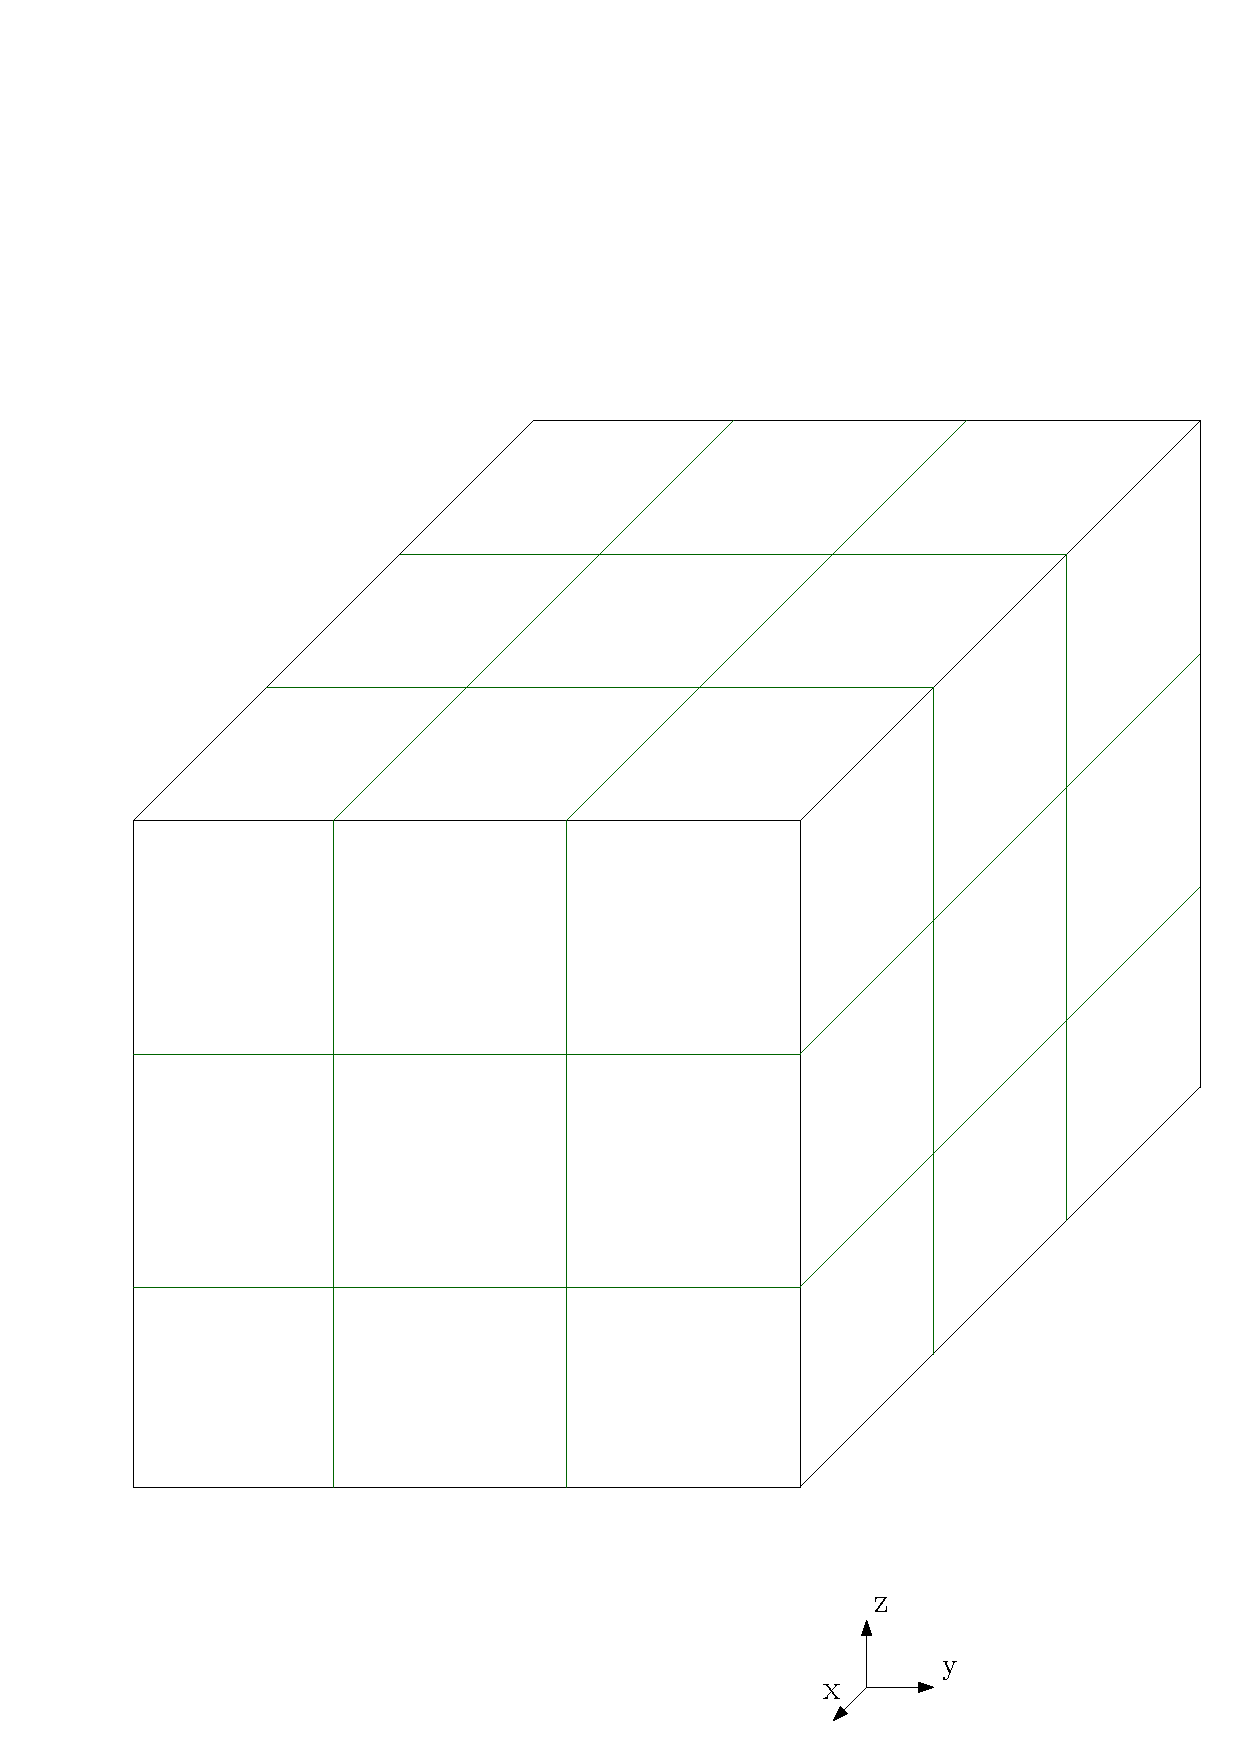
\includegraphics[scale=0.5]{MPI_cubic_division}
	\caption{Schematic representation of the grid separation in the case of a cubic number of processes.}
	\label{fig:CUBICSEPARATION}
\end{figure}
%
The numbering of the different processes in thois case is first along the \textit{x}-axis, then along the \textit{y}-axis and finally along the \textit{z}-axis, meaning that processes $0,1,\cdots,N-1$ are along the \textit{x}-axis, then the processes $N, N+1,\cdots,2*N-1$ are also along the \textit{x}-axis, but one "step" further along the \textit{y}-axis. We continue the numbering until we are at the extremity of the \textit{y}-axis. Once the first stage is filled, we increase the height and reiterate the numbering from $N^2$.

\subsection{Even number of processes}
If the number of processes is not cubic, the parity of this number is checked. If it is even, the division into subgrids is represented in \Cref{fig:EVENSEPARATION}.
%
\begin{figure}
    \centering
    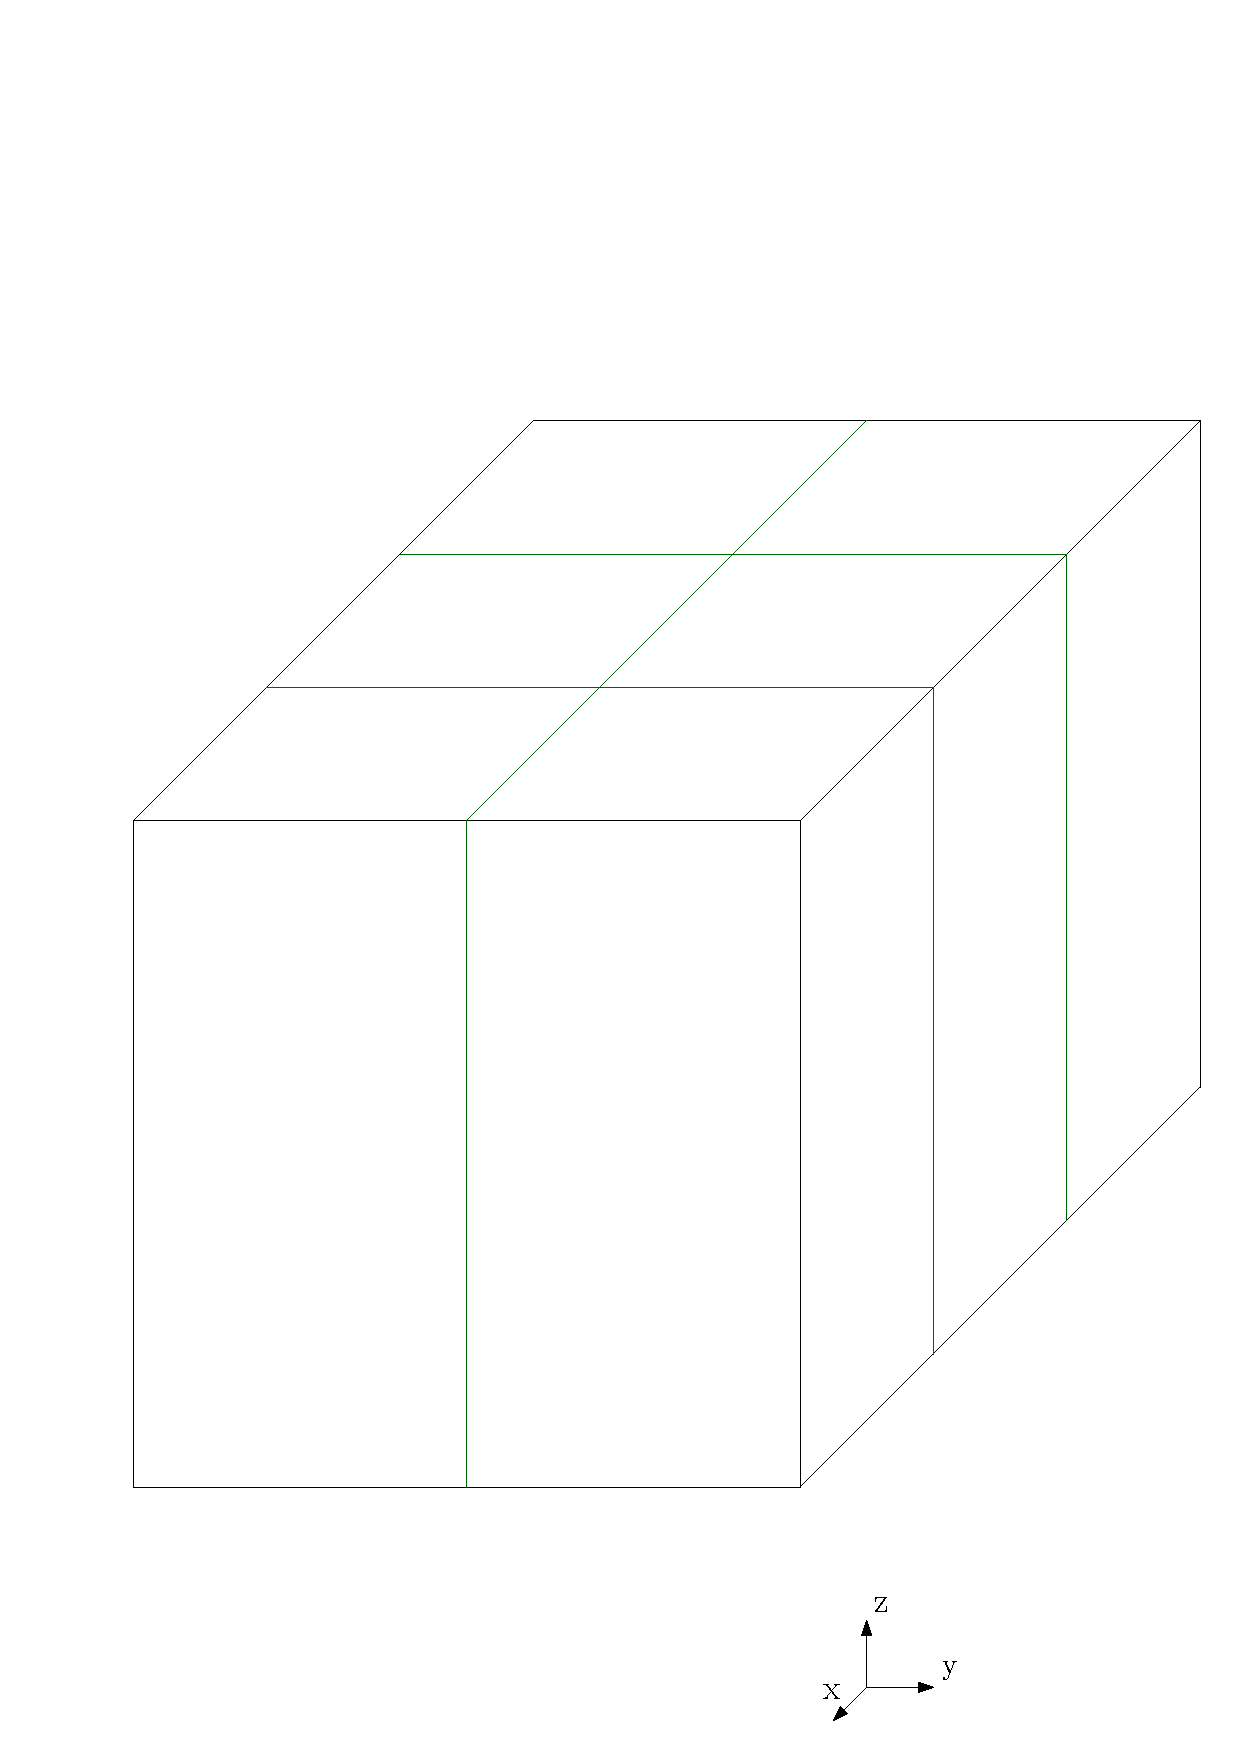
\includegraphics[scale=0.5]{MPI_pair_division}
    \caption{Schematic representation of the grid separation in the case of an even number of processes.}
    \label{fig:EVENSEPARATION}
\end{figure}
%
The methodology is as follow : the initial grid is first cut into 2 subgrids along the \textit{xz}-midplane. If there are only 2 processes, the subdivision is finished. If there are more, the grid is further cut along parallel \textit{yz}-planes.

\subsection{Odd number of processes}
If the number of processes is neither cubic, nor even, it is odd. In this case, the division is depicted in \Cref{fig:ODDSEPARATION}.
%
\begin{figure}
    \centering
    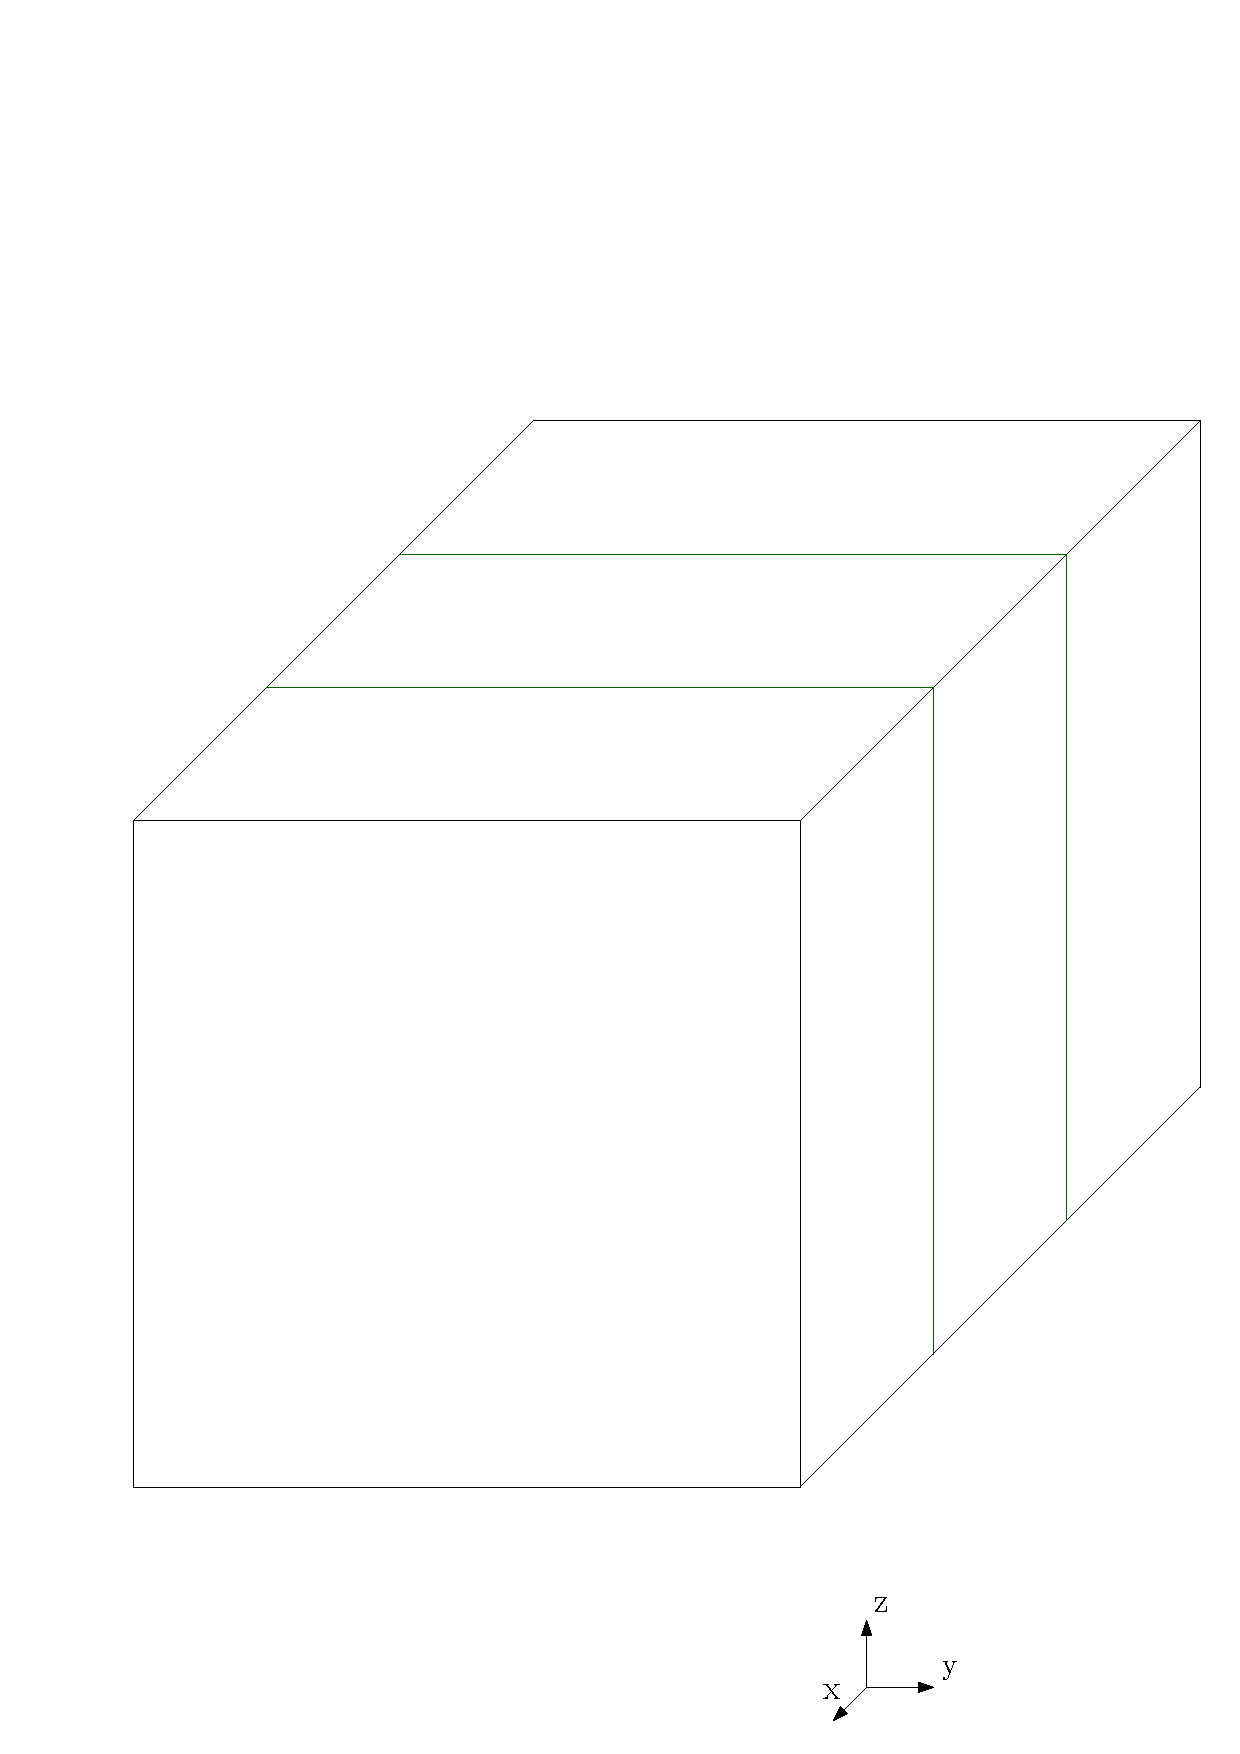
\includegraphics[scale=0.5]{MPI_impair_division}
    \caption{Schematic representation of the grid separation in the case of an odd number of processes.}
    \label{fig:ODDSEPARATION}
\end{figure}
%
As can be seen in this picture, the subgrids are made by cutting the initial grid with \textit{yz}-planes. The number of separations is obtained by considering that each division is one process.




\section{Explanation of the test cases}
\subsection{Thin wire}
As was previously said, the study case here is that of a thin wire only excited by only an electric field along one direction. As can be seen in \Cref{fig:THINWIRE}, the magnetic field generated in such a configuration is consistent with the physical intuition.
%
\begin{figure}
	\centering
	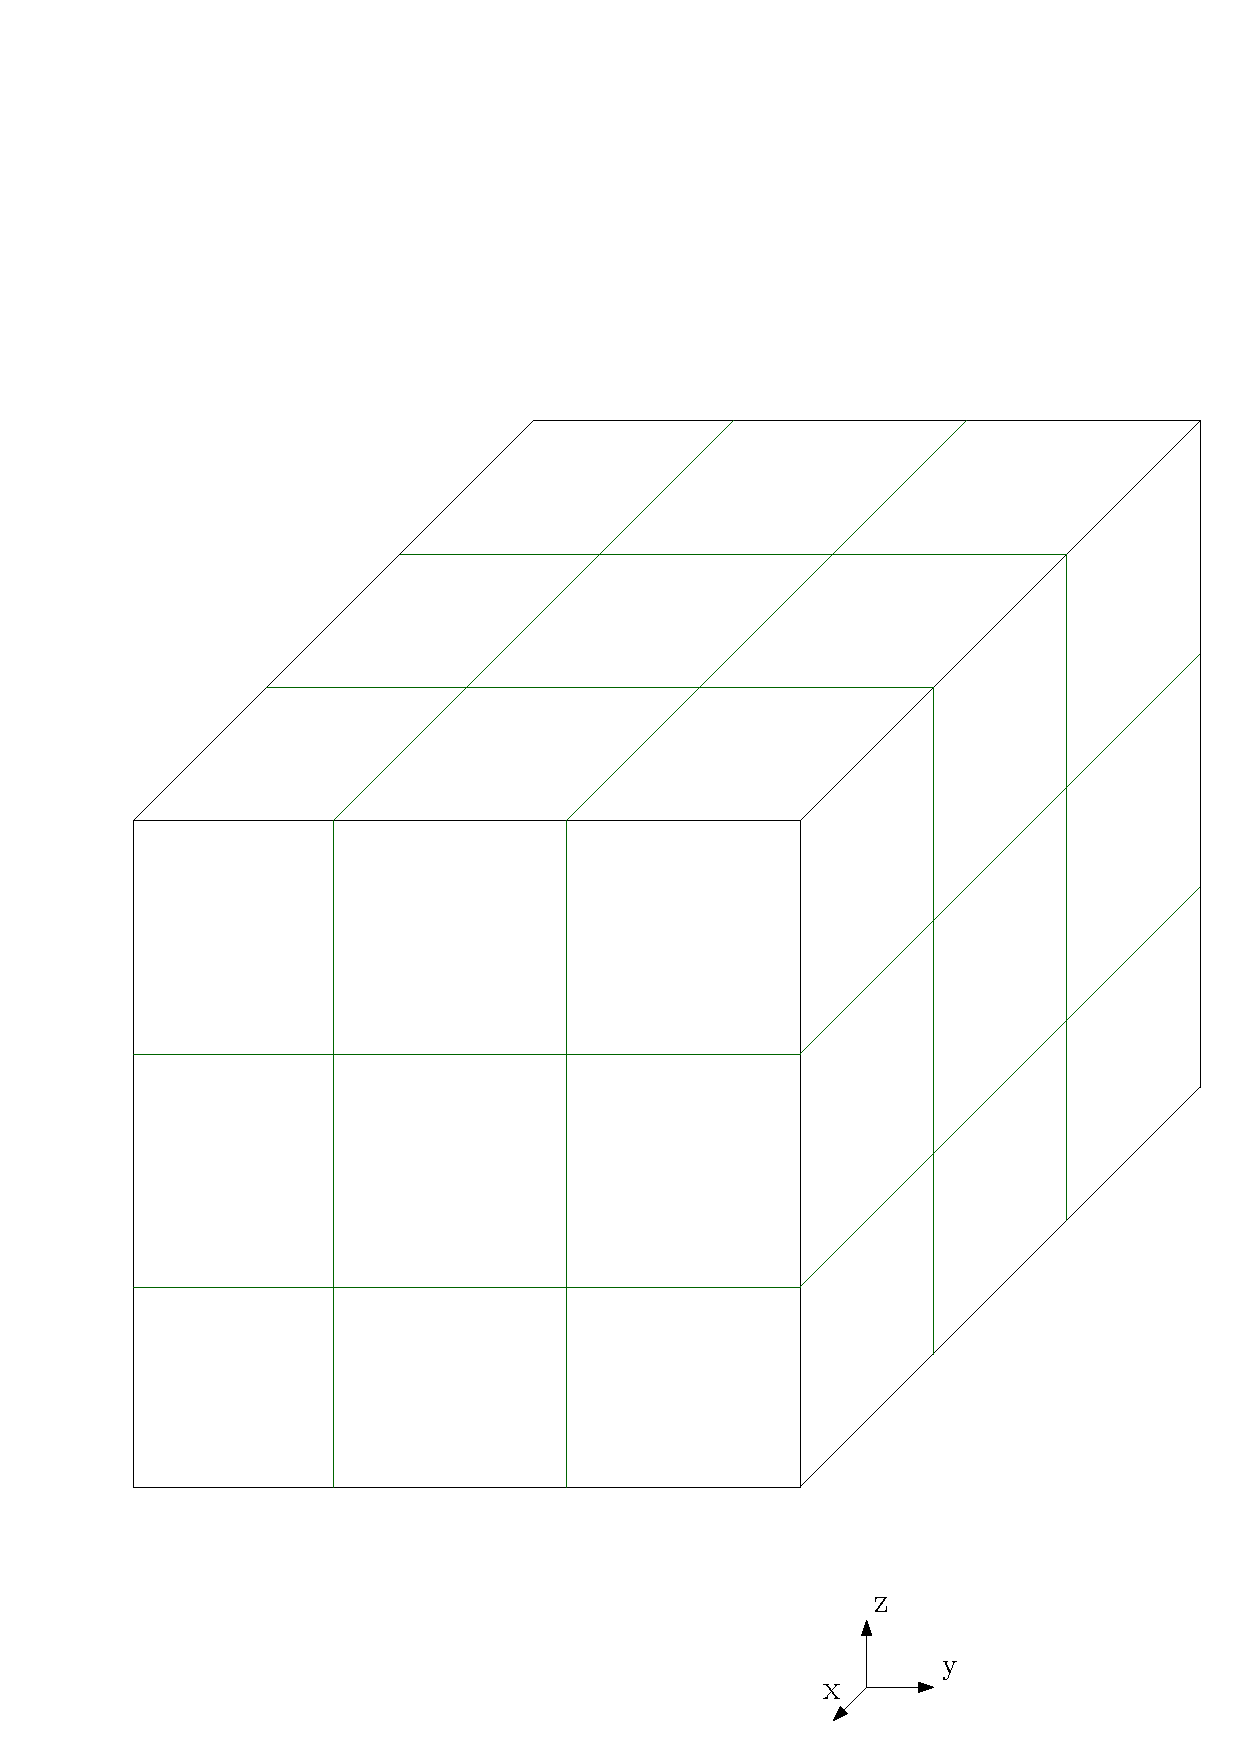
\includegraphics[scale=0.5]{MPI_cubic_division}
	\caption{Results for the thin wire excited by a one-component electric field.}
	\label{fig:THINWIRE}
\end{figure}
%


\subsection{Dipole antenna}
Here, a dipole antenna is studied, but its air gap has a null dimension, meaning that the antenna is just a source. On this source, only a component of the electric field is set to a certain value whereas all the others are iposed to zero. Concerning the magnetic fields, their values are updated by using the classical 3 dimensional YEE algorithm. The results are visible in \Cref{fig:DIPOLEANTENNA}.
%
\begin{figure}
	\centering
	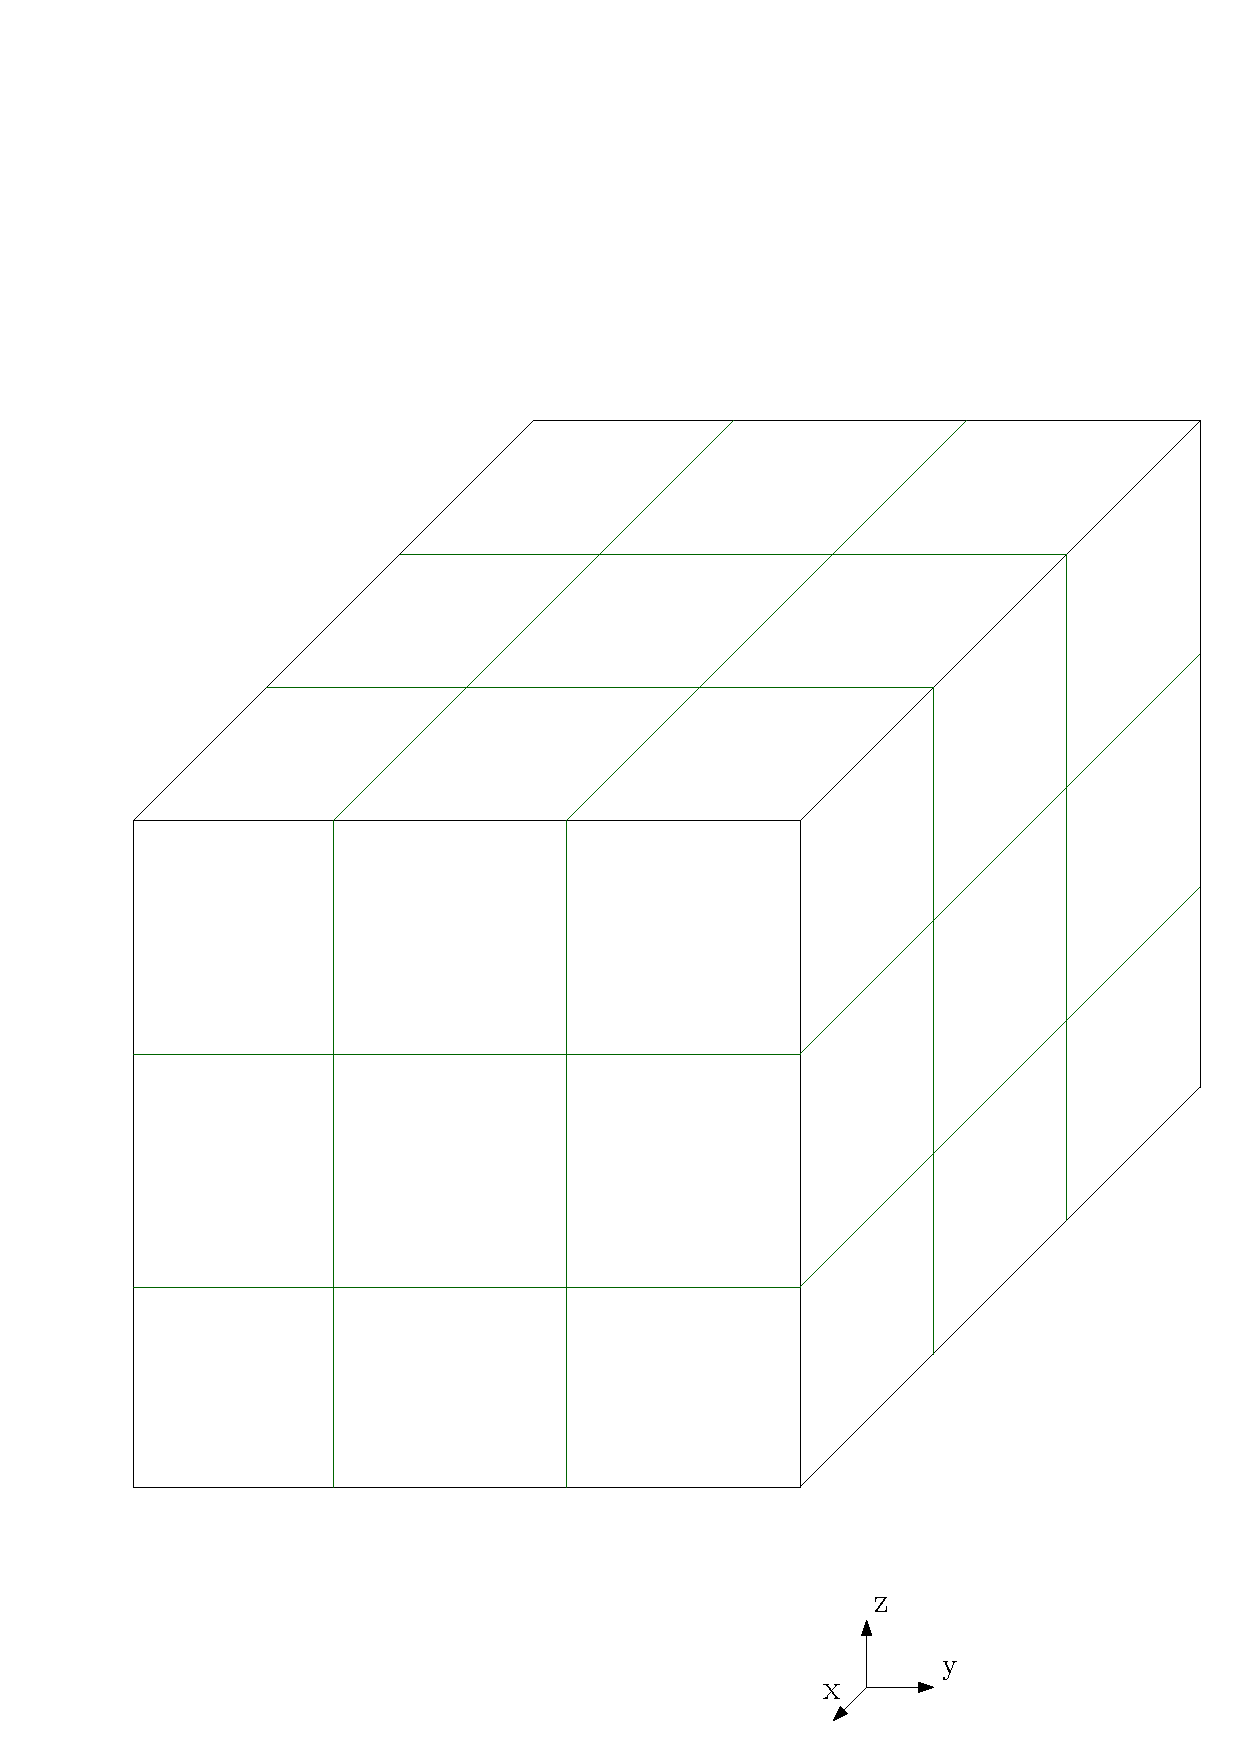
\includegraphics[scale=0.5]{MPI_cubic_division}
	\caption{Results for the dipole antenna with a zero air gap.}
	\label{fig:DIPOLEANTENNA}
\end{figure}
%



\end{document}
